\documentclass[12pt]{article}
\usepackage{graphicx,url}
\usepackage[a4paper,margin=1in]{geometry}
\usepackage[super,sort&compress,comma]{natbib}
\usepackage[breaklinks=true,colorlinks=true,linkcolor=blue,urlcolor=blue,citecolor=blue]{hyperref}
\usepackage{siunitx}
\usepackage{hyperref}
\usepackage{booktabs}
\usepackage{floatrow}
\usepackage{subcaption}
\usepackage{paralist}
\usepackage{listings}
\usepackage{authblk}
\usepackage[normalem]{ulem}
\usepackage{xcolor}
\usepackage{amsmath}
\usepackage{amssymb}
\usepackage{amsthm}
\usepackage{gensymb}
\usepackage{enumitem}
\usepackage{textgreek}
\usepackage{algorithm}
\usepackage{algpseudocode}
\usepackage[flushleft]{threeparttable}
\usepackage{threeparttablex}

\graphicspath{ {FIGURES/} } % Folder containing images
\renewcommand{\thepage}{S\arabic{page}}
\renewcommand{\thesection}{S\arabic{section}}
\renewcommand{\thetable}{S\arabic{table}}
\renewcommand{\thefigure}{S\arabic{figure}}
\newcommand{\jon}[1]{{\color{red}#1}}
\newcommand{\amanda}[1]{{\color{green}#1}}


\begin{document}

\title{ From Molecular Dynamics to Machine Learning:\\ Extracting Data via Iterative Archetypal Analysis  \linebreak  SUPPORTING INFORMATION }
\author[1]{Jonathan Y. C. Ting \footnote{Corresponding author: jonathan.ting@anu.edu.au}}
\author[1]{Amanda S. Barnard \footnote{Corresponding author: amanda.s.barnard@anu.edu.au}}
\affil[1]{School of Computing, Australian National University, Acton 2601, Australia}
\date{}
\setcounter{Maxaffil}{0}
\renewcommand\Affilfont{\itshape\small}

\maketitle



\section{Archetypal Analysis Acceleration}
\label{sec:SIAAaccelerate}


Careful initialisation of the coefficient matrices is recognised as an important factor in accelerating convergence and avoiding degenerate archetypes, particularly ensuring that the initial archetypes are well separated from one another. Two initialisation procedures that operate before the alternating minimisation step have been proposed: \texttt{FurthestSum}~\cite{Morup2012kernelAA} and \texttt{AA++}~\cite{Mair2023AA++}. The \texttt{FurthestSum} heuristic is adapted from the \texttt{FurthestFirst} strategy used in $k$-means initialisation~\cite{Hochbaum1985FurtherFirst}, while \texttt{AA++} is a probabilistic scheme that draws candidate archetypes sequentially in proportion to their influence on the objective function, analogously to \texttt{$k$-means++}~\cite{Mair2023AA++}.

Coresets are compact weighted subsets of a dataset constructed so that any algorithm run on the coreset achieves performance provably close to that obtained on the full data~\cite{Feldman2020coresets}. When a coreset is a sufficiently faithful representation of the original data, AA applied to the coreset yields results comparable to full-data AA, but at substantially lower computational cost. Mair \textit{et al.} developed a coreset construction procedure that requires only two passes through the data~\cite{Mair2019Coresets} and provides a formal bound on the resulting approximation error, guaranteeing that the quality of results on the coreset is competitive with the full-data solution. The coreset approach has been argued to be among the most theoretically rigorous options for approximating AA~\cite{Mair2019Coresets}.

IAA shares conceptual ground with the coreset method~\cite{Mair2019Coresets} in that both involve extracting a smaller set of samples from the original data and performing the main computation on that reduced set, making both methods approximate in nature. However, the two approaches differ in important respects. In IAA, the intermediate samples returned by AA on each subset need not correspond to any configuration actually present in the original data (they are hypothetical by construction) and they do not currently satisfy the mathematical requirements for coreset membership. In terms of the number of data passes required, the coreset method (which needs only two passes) is arguably more economical than IAA. Nevertheless, the highly parallel structure of IAA can offer faster wall-clock times for the subset identification step when datasets are very large.
IAA should also be distinguished from the geometry-based approach of Abrol and Sharma~\cite{Abrol2020GeomAA}, despite both methods framing their contributions in terms of the geometric structure of the AA problem. Similarly, the word ``iterative'' appears in both names but refers to distinct stages: in the geometric method, iteration applies to the subset selection procedure, whereas in IAA it refers to successive rounds of AA.



\section{Conventional Domain-Driven Sample Reduction}
\label{sec:SISampleReduction}

As noted in the main text, a domain-driven strategy for detecting and removing redundant conformations was applied during the sampling phase of the MD simulations. The overall workflow for this procedure is illustrated in Fig.~\ref{fig:sampleReductionWorkflow}.
\begin{figure}[!ht]
    \centering
    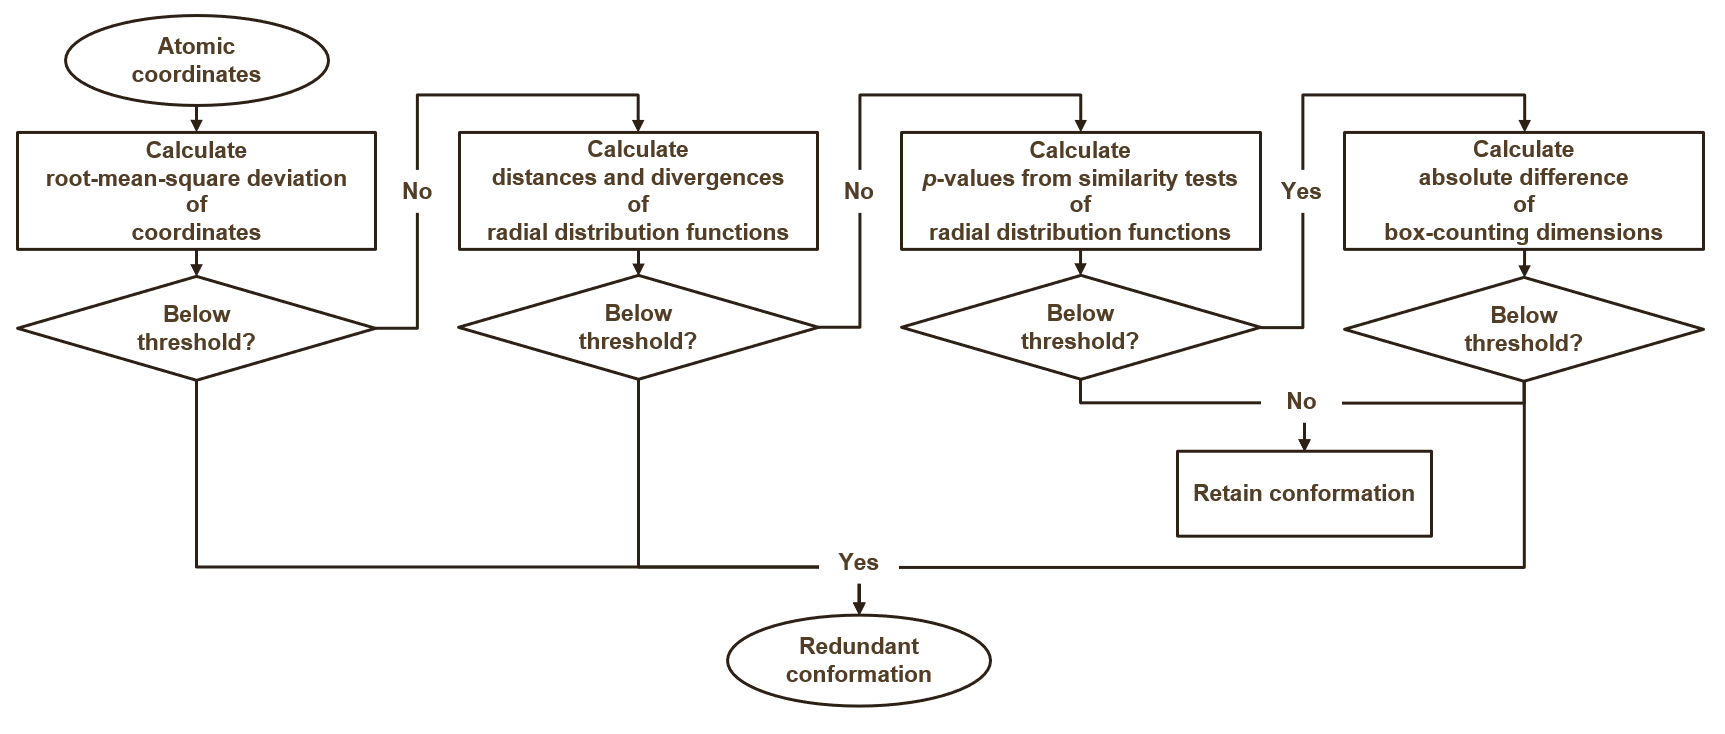
\includegraphics[width=\textwidth]{sampleReductionWorkflow}
    \caption{Overview of the workflow of the identification of redundant nanoparticle conformations.}
    \label{fig:sampleReductionWorkflow}
\end{figure}

The threshold for each similarity metric was calibrated by monitoring how that metric changes over the course of melting simulation trajectories for a representative selection of nanoparticles. For a given pair of conformations, the first is classified as redundant if and only if all of the following conditions are met simultaneously:
\begin{enumerate}
    \item the root mean squared error between the atomic coordinates of the two conformations falls below a threshold (set to 0.05 \AA),
    \item the mutual information~\cite{Kreer1957MI,Shannon1948MI} between the average bond length distributions of the two conformations exceeds a threshold (set to 1.0),
    \item the \textit{p}-values from the 2-sample Anderson-Darling test~\cite{Scholz2012ADtest}, 2-sample Kolmogorov-Smirnov test~\cite{Conover1965KStest}, and 2-sample Cram\'er-von Mises test~\cite{Anderson1962CMtest} applied to the pair of radial distribution functions all exceed the standard significance level (set to 0.05),
    \item the Hellinger distance, Jensen-Shannon divergence, and Kantorovich-Rubinstein metric between the radial distribution functions of the two conformations each fall below their respective thresholds (set to 0.08, 0.005, and 0.0001), and
    \item the Kullback-Leibler divergence from the radial distribution function of the first conformation to that of the second conformation is less than a threshold (set to 0.25); note that this measure is asymmetric, i.e.\ $KL(P, Q) \neq KL(Q, P)$.
\end{enumerate}

For the bimetallic datasets, a reduced set of similarity metrics was used to balance computational cost against the breadth of information captured. Specifically, two metrics from the full pipeline were omitted: the mutual information of the average bond length distributions, and the Kullback-Leibler divergence of the RDF of the current conformation from that of the previous conformation. The thresholds applied to the remaining metrics are as follows:
\begin{enumerate}
    \item root-mean-square deviation (computed in Euclidean distance) between the current and previous conformations (threshold of $1.0$),
    \item Wasserstein distance~\cite{Kantorovich1960KantorovichDist} (threshold of $0.0002$), Hellinger distance~\cite{Beran1977HellingerDist} (threshold of $0.15$), and Jensen-Shannon divergence~\cite{Fuglede2004JSdiv} between the RDF of the current and previous conformations (threshold of $0.02$), and
    \item \textit{p}-values (with thresholds of 0.05) from the 2-sample Anderson-Darling test, 2-sample Kolmogorov-Smirnov test, and 2-sample Cram\'er-von Mises test, each testing the null hypothesis that the radial distribution functions of the current and previous conformations are drawn from the same distribution.
\end{enumerate}



\section{Metal Nanoparticle Datasets}
\label{sec:rawDatasets}

\begin{table}[htbp!]
\caption{Descriptions of the metal nanoparticle data sets used in the main text. Domain-driven reduction was applied only to bimetallic instances, using the methods described in Section~\ref{sec:SISampleReduction}. The ranges of atom number and nanoparticle diameter were unchanged by the reduction.}
\centering
\small
    \begin{tabular}{c|ccccc|cc}
            \hline
            Data            & Number   & Original  & Minimum   & Minimum  & Reference                & Final     & Percentage \\
            set             & of       & Number    & and       & and      & to public                & Number    & of         \\
                            & features & of        & maximum   & maximum  & repository               & of        & reduction  \\
                            &          & instances & atom      & diameter &                          & instances\tnote{a} & ($\%$)     \\
                            &          &           & number    & (nm)     &                          &           &            \\
            \hline
            Au      &      182 &      4000 & 236-14277 &  1.7-7.8 & \cite{Barnard2019AuData} &           - &        - \\
            Pd      &      182 &      4000 & 137-16262 &  1.4-7.5 & \cite{Barnard2019PdData} &           - &        - \\
            Pt      &      182 &      1300 &  54-15837 &  1.5-7.6 & \cite{Barnard2019PtData} &           - &        - \\
            AuPd    &      922 &    145103 &   93-4631 &  1.1-5.1 &  \cite{Ting2023AuPdData} &       47623 &     67.2 \\
            AuPt    &      922 &    162439 &   93-4631 &  1.1-5.1 &  \cite{Ting2023AuPtData} &       53445 &     67.1 \\
            PdAu    &      922 &    145064 &  105-4631 &  1.2-5.0 &  \cite{Ting2023PdAuData} &       48087 &     66.9 \\
            PdPt    &      922 &    151216 &  105-4631 &  1.2-5.0 &  \cite{Ting2023PdPtData} &       48785 &     67.7 \\
            PtAu    &      922 &    162770 &  105-4631 &  1.2-5.1 &  \cite{Ting2023PtAuData} &       54006 &     66.8 \\
            PtPd    &      922 &    150781 &  105-4631 &  1.2-5.0 &  \cite{Ting2023PtPdData} &       48943 &     67.5 \\
            AuPdPt  &     1958 &     48136 &   603-959 &  2.3-2.9 &  \cite{Lu2023AuPdPtData} &           - &        - \\
            \hline
    \end{tabular}
    \label{tab:rawDatasets}
\end{table}

\section{IAA Parameters for Metal Nanoparticle Datasets}
\label{sec:SIIAAparams}

Table~\ref{tab:redRedAppendixIAAparams} lists the complete set of IAA parameters used for sample redundancy reduction of the metal nanoparticle datasets described in the main text. The number of subsets was chosen to guarantee that each subset is large enough to support the extraction of the specified number of archetypes during the elbow plot analysis, where $p_1$ and $p_2$ were held equal. For the monometallic dataset, each subset must contain more samples than the maximum archetype count explored in the elbow analysis (300); since the monometallic dataset has 9300 samples in total, dividing it into 100 subsets of only 93 samples each would be inappropriate. For IAA runs targeting the maximum archetype count ($p_2$=5000) and for runs without redundant archetypes, the largest available $p_1$ values are used, as the results in Section~\ref{sec:SIRandomVsElementSplitting} indicate that a larger number of intermediate archetypes improves the retention of explained variance across subset AA rounds.

\begin{table}[htbp!]
\caption{Parameters of iterative archetypal analysis for the monometallic, bimetallic, and trimetallic nanoparticle datasets, including the number of subsets ($k$), number of intermediate archetypes ($p_1$), and number of final archetypes ($p_2$).}
\centering
\small
\begin{tabular}{cc|ccc}
\hline
IAA runs with                  & Parameters &  Monometallic &  Bimetallic &  Trimetallic \\
\hline
Elbow plot-informed archetypes & $k$        &   10 &  100 &   10 \\
                               & $p_1$      &  100 &  200 &  200 \\
                               & $p_2$      &  100 &  200 &  200 \\
Maximum number of archetypes   & $k$        &   10 &  100 &   10 \\
                               & $p_1$      &  300 &  500 & 1000 \\
                               & $p_2$      & 5000 & 5000 & 5000 \\
No redundant archetype         & $k$        &   10 &  100 &   10 \\
                               & $p_1$      &  300 &  500 & 1000 \\
                               & $p_2$      &  250 & 1800 & 3000 \\
\hline
\end{tabular}
\label{tab:redRedAppendixIAAparams}
\end{table}



\section{Comparisons between Random and Element-Based Splitting}
\label{sec:SIRandomVsElementSplitting}

Several strategies can be used to partition the original dataset into subsets for IAA. Here, splitting based on nanoparticle elemental composition (a form of domain knowledge) is compared with random splitting, with all other parameters held fixed. For this comparison, $p_1$ and $p_2$ are set equal. As shown in Fig.~\ref{fig:MNP3S_split_expVar}, elemental composition-based splitting consistently achieves higher explained variance than random splitting. For random splitting, increasing the number of subsets tends to improve explained variance when more than 200 archetypes are extracted, because more subsets increase the probability that individual subsets span regions requiring a larger number of archetypes to explain their variance.

\begin{figure}[htbp]
    \centering
    \begin{subfigure}{0.4\textwidth}
        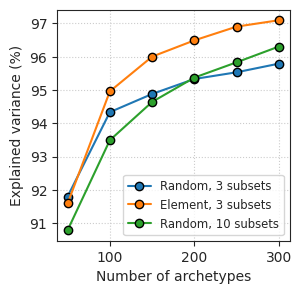
\includegraphics[width=\textwidth]{MNP_split_all_expVar}
        \caption{} \label{fig:MNP_split_all_expVar}
    \end{subfigure}
    \begin{subfigure}{0.41\textwidth}
        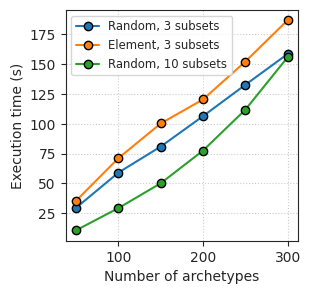
\includegraphics[width=\textwidth]{MNP_split_all_exeTime}
        \caption{} \label{fig:MNP_split_all_exeTime}
    \end{subfigure}
    \caption{(a) Explained variance from iterative archetypal analysis with different number of archetypes, with subset selection \textit{via} either random or element-based splitting, and (b) the execution time.}
    \label{fig:MNP3S_split_expVar}
\end{figure}

For visualisation of high-dimensional data in two dimensions, \textit{t}-SNE as implemented in \texttt{scikit-learn} is used, with the following parameter settings: \texttt{n\_components}=2, \texttt{perplexity}=30.0, \texttt{early\_exaggeration}=12.0, \texttt{learning\_rate}=`auto', \texttt{n\_iter}=1000, \texttt{n\_iter\_without\_progress}=300, \texttt{min\_grad\_norm}=$1 \times 10^{-7}$, \texttt{metric}=metric, \texttt{random\_state}=42, \texttt{init}=`pca', \texttt{method}=`barnes\_hut', and \texttt{angle}=0.5. Comparing the archetype distributions from random and elemental splitting in Fig.~\ref{fig:MNP3S_split_closeMatch_tSNE}, the element-based approach places fewer archetypes in the lower-left region of the \textit{t}-SNE embedding. Given that elemental splitting also yields higher explained variance, this suggests that the samples in that region are largely similar to one another and can be adequately represented by a small number of archetypes, freeing the remaining archetypes to account for variance in the rest of the feature space.

\begin{figure}[htbp] \centering
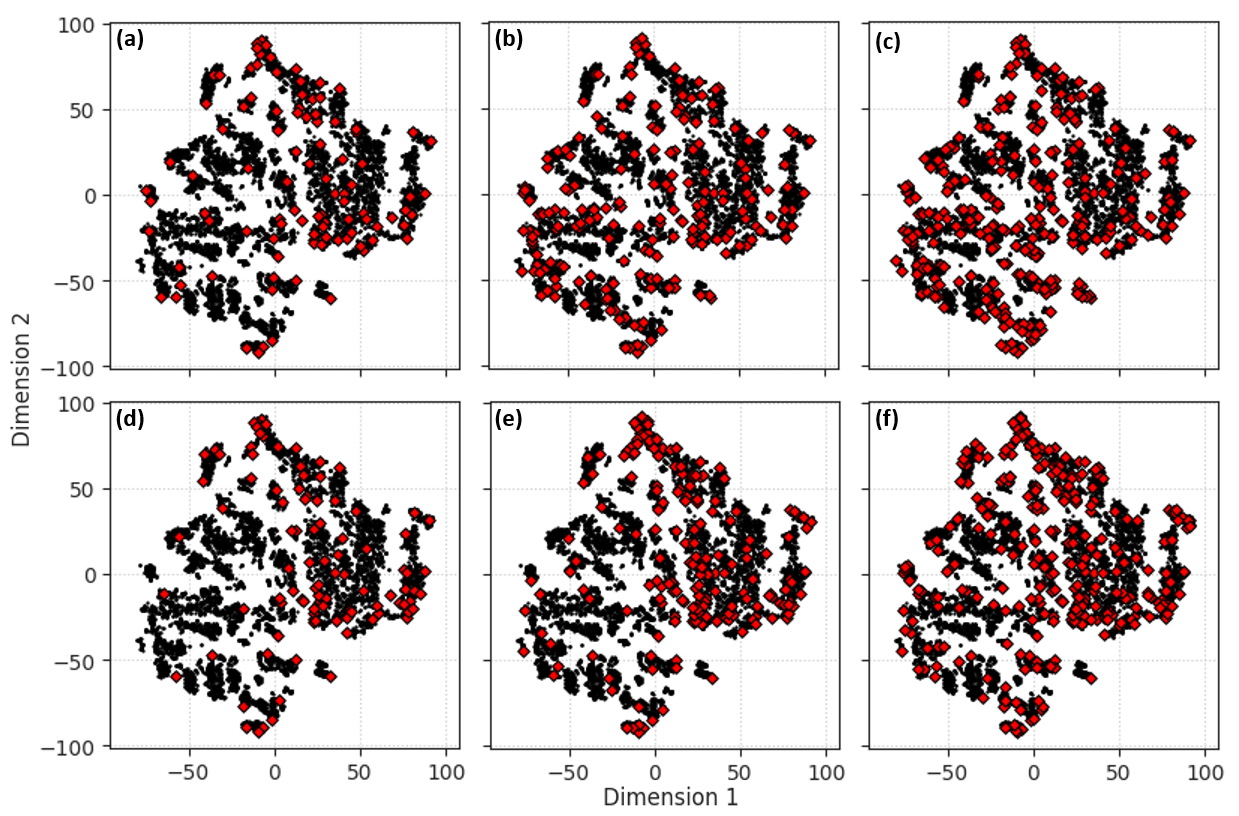
\includegraphics[width=\textwidth]{MNP3S_split_closeMatch_tSNE}
\caption{Mapping of the samples (black dots) and archetypes (red stars) of the monometallic nanoparticle dataset onto 2D embedded space learnt \textit{via} \textit{t}-distributed stochastic neighbour embedding, with (a, d) 100, (b, e) 200, and (c, f) 300 archetypes obtained from (a-c) random and (d-f) element-based splitting with 3 subsets. The reduced dimensions are arbitrary.}
\label{fig:MNP3S_split_closeMatch_tSNE}
\end{figure}

Although element-based splitting outperforms random splitting in this case, this advantage does not generalise unconditionally. Elemental composition splitting cannot be applied to datasets containing only a single elemental combination, such as the trimetallic dataset. Likewise, partitioning based on continuous variables such as nanoparticle size would require an arbitrary threshold to define categories. For these reasons, random splitting is used for all metal nanoparticle datasets throughout this work.

Figures~\ref{fig:MNP3S_randomSplit_closeMatch_tSNE}, \ref{fig:MNP3S_eleSplit_closeMatch_tSNE}, and \ref{fig:MNP10S_randomSplit_closeMatch_tSNE} show how the sample and archetype distributions in the monometallic dataset vary across splitting strategies and subset counts.
\begin{figure}[htbp] \centering
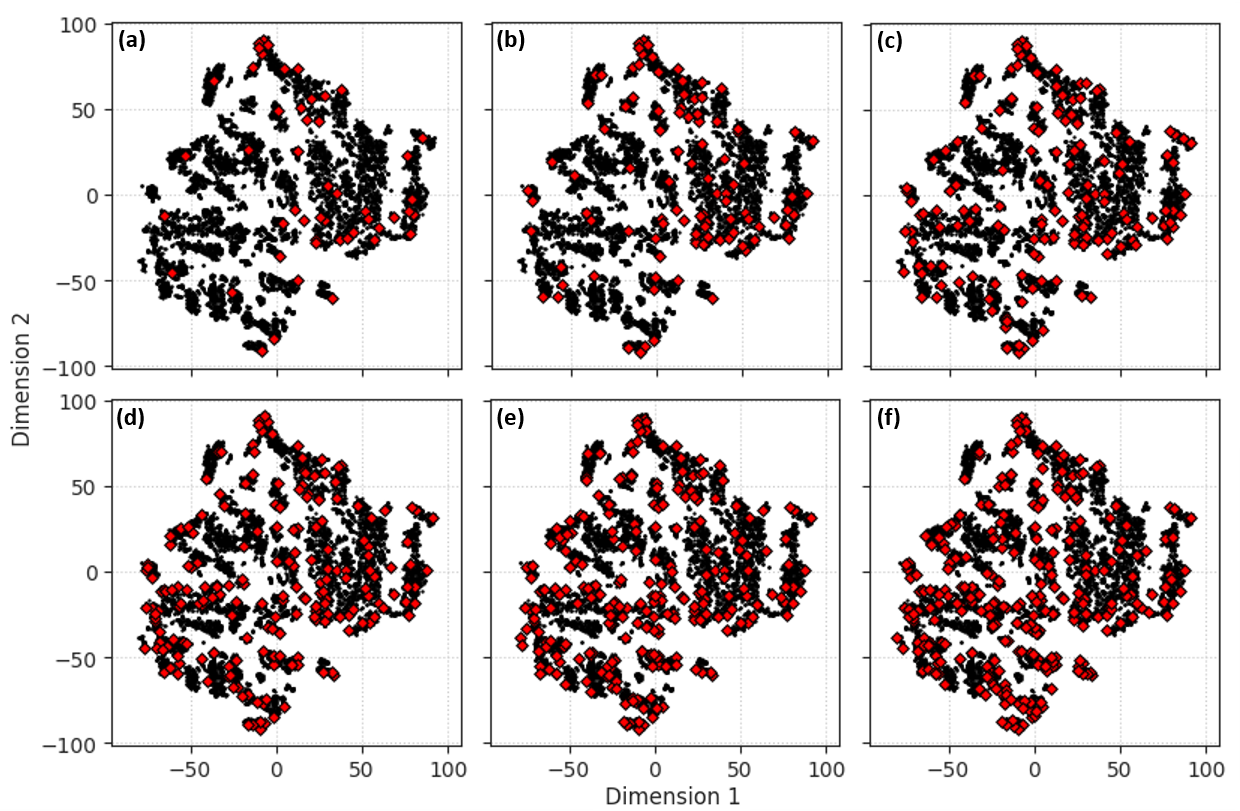
\includegraphics[width=\textwidth]{MNP3S_randomSplit_closeMatch_tSNE}
\caption{Mapping of the samples (black dots) and archetypes (red stars) obtained from random splitting of the monometallic nanoparticle dataset into 3 subsets onto 2D embedded space learnt \textit{via} \textit{t}-distributed stochastic neighbour embedding. The reduced dimensions are arbitrary.}
\label{fig:MNP3S_randomSplit_closeMatch_tSNE}
\end{figure}

\begin{figure}[htbp] \centering
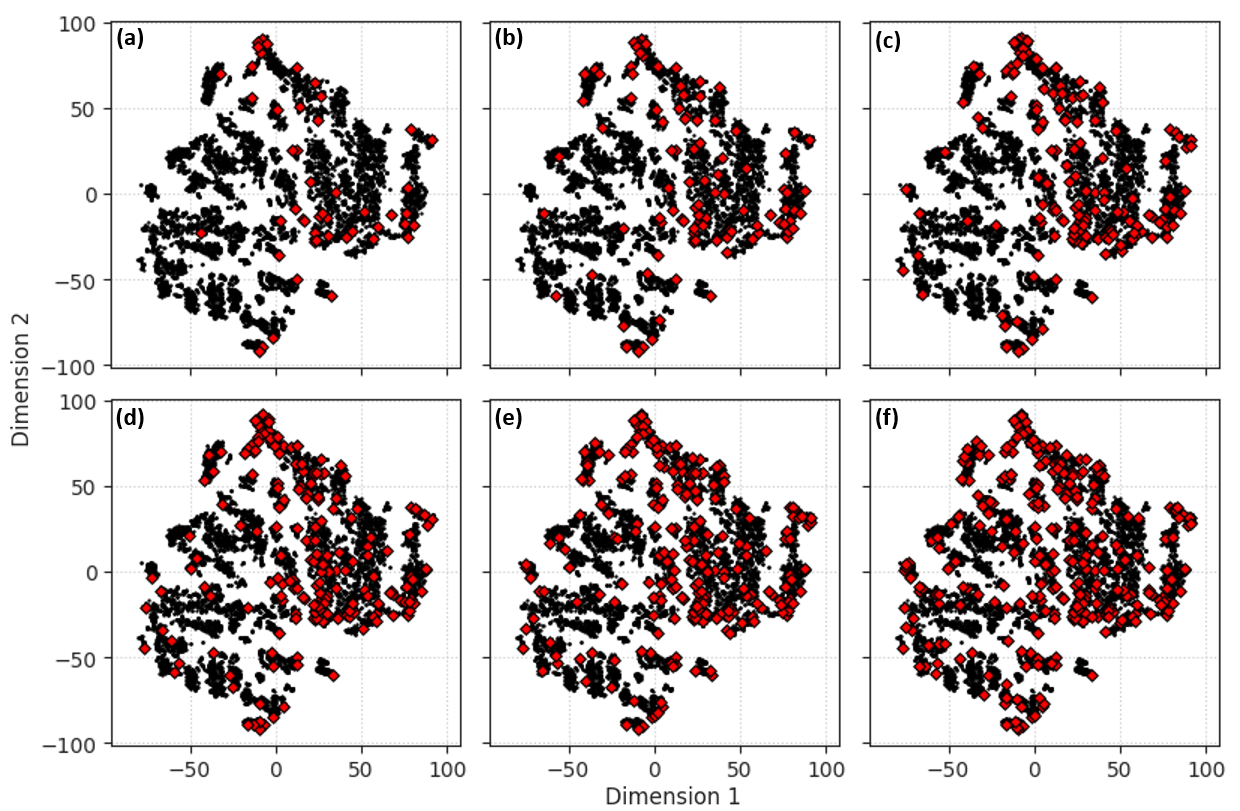
\includegraphics[width=\textwidth]{MNP3S_eleSplit_closeMatch_tSNE}
\caption{Mapping of the samples (black dots) and archetypes (red stars) obtained from element-based splitting of the monometallic nanoparticle dataset into 3 subsets onto 2D embedded space learnt \textit{via} \textit{t}-distributed stochastic neighbour embedding. The reduced dimensions are arbitrary.}
\label{fig:MNP3S_eleSplit_closeMatch_tSNE}
\end{figure}

\begin{figure}[htbp] \centering
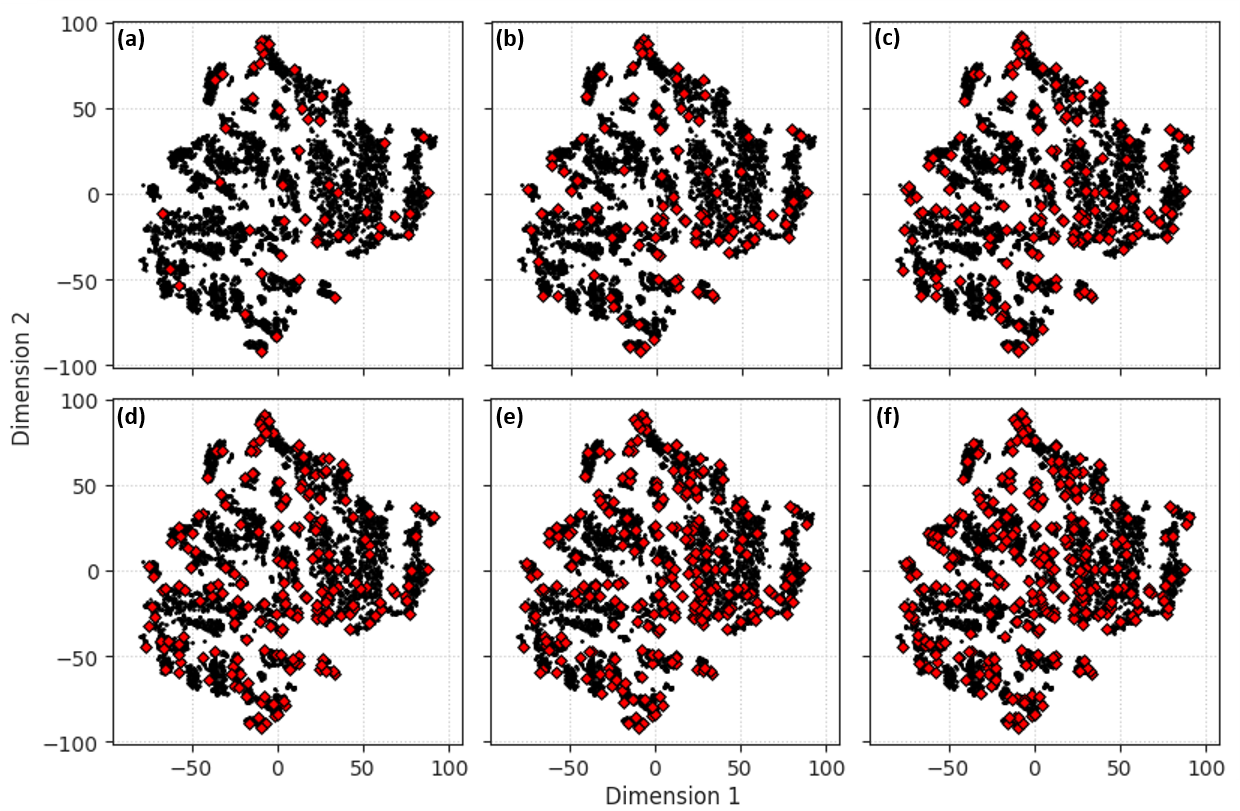
\includegraphics[width=\textwidth]{MNP10S_randomSplit_closeMatch_tSNE}
\caption{Mapping of the samples (black dots) and archetypes (red stars) obtained from random splitting of the monometallic nanoparticle dataset into 10 subsets onto 2D embedded space learnt \textit{via} \textit{t}-distributed stochastic neighbour embedding. The reduced dimensions are arbitrary.}
\label{fig:MNP10S_randomSplit_closeMatch_tSNE}
\end{figure}



\clearpage
\section{Optimising the Numbers of Archetypes}
\label{sec:SINumArchOpt}

As described in the main text, the appropriate number of archetypes is determined by starting from 5000 (a value known to produce redundant sampling) and progressively reducing this number until the vertices of the simplex plots are fully or nearly populated by configurations that are present in the original dataset. Representative examples of this process are shown in Fig.~\ref{fig:BTNPsNumArchs}. Notably, the prototype in Fig.~\ref{fig:BTNPsNumArchs}(d) is positioned closer to the centre than those in panels (e) and (f), illustrating that a central prototype position is not sufficient to confirm the absence of redundant archetypes.

\begin{figure}[htbp] \centering
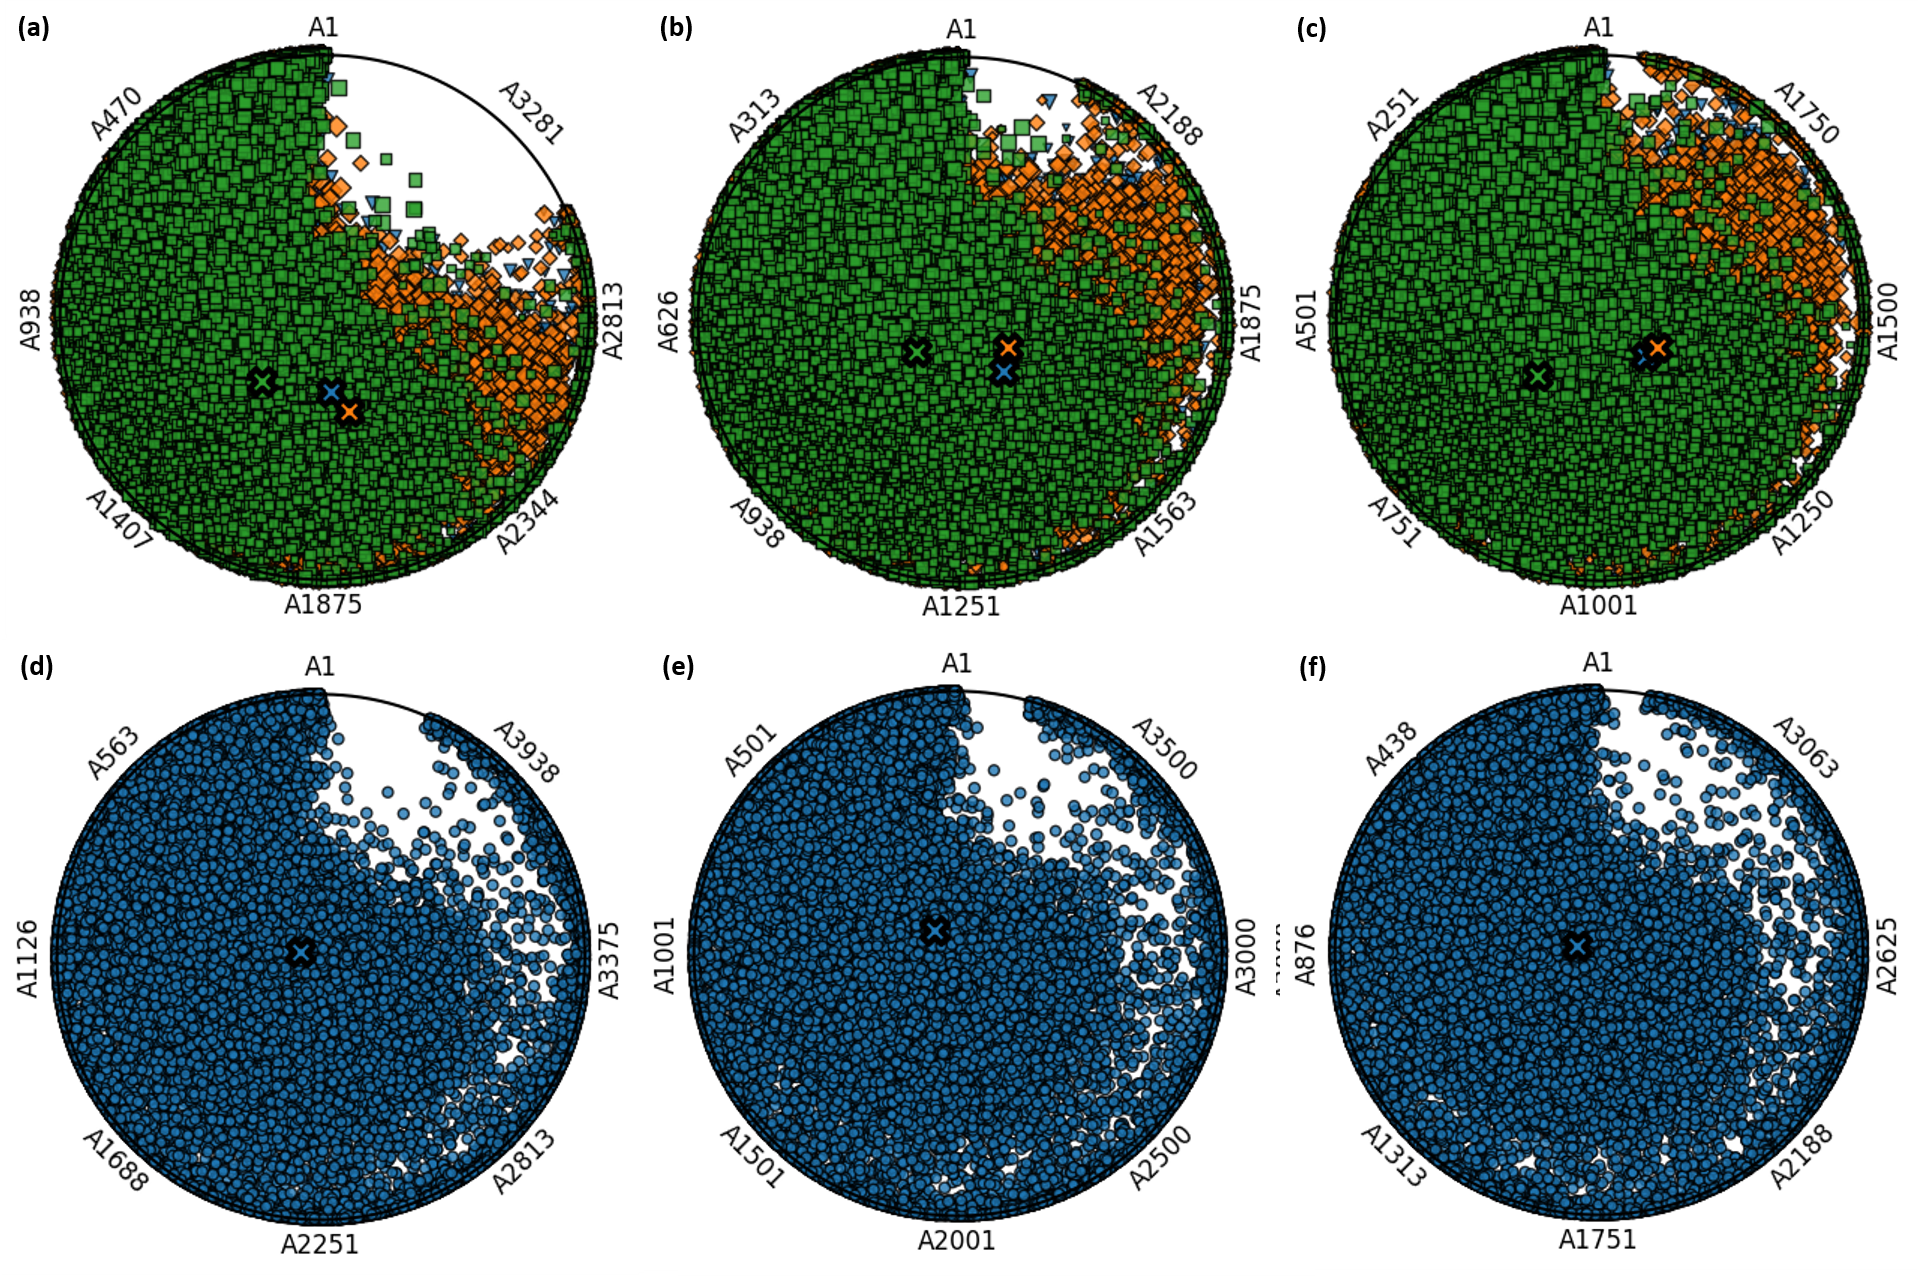
\includegraphics[width=\textwidth]{BTNPsNumArchs}
\caption{Simplex plots of the samples for bimetallic AuPd (blue), AuPt (orange), and PdPt (green) nanoparticle datasets with (a) 5000, (b) 2500, and (c) 2000 archetypes, and trimetallic AuPdPt (blue) nanoparticle dataset with (d) 5000, (e) 3750, and (f) 3500 archetypes. The crosses indicate the hypothetical prototypes with averaged feature values and the same elemental combinations. Points are sized relative to the average diameters of the nanoparticles.}
\label{fig:BTNPsNumArchs}
\end{figure}



\clearpage
\section{Contribution from Archetypes to Data Samples}
\label{sec:SIContribArch2Sam}

Figure~\ref{fig:allNPs_maxArchs_compareCloseMatch} compares the archetypal contributions to the nearest original samples for archetypes drawn from populated versus unpopulated simplex regions. Archetypes located outside the mainly empty sectors contribute substantially to their closest samples, whereas those residing within the empty sectors contribute negligibly even to the samples nearest to them. This pattern confirms that the selection of 5000 archetypes leads to a poorly representative sampling of the original datasets. Further evidence of this over-parameterisation is provided in Fig.~\ref{fig:allNPs_maxArchs_compareArchContribRadarPlots}, which displays contribution radar plots across 100 randomly selected samples and shows that the higher-indexed archetypes account for virtually no variance in any of them.
\begin{figure}[htbp!] \centering
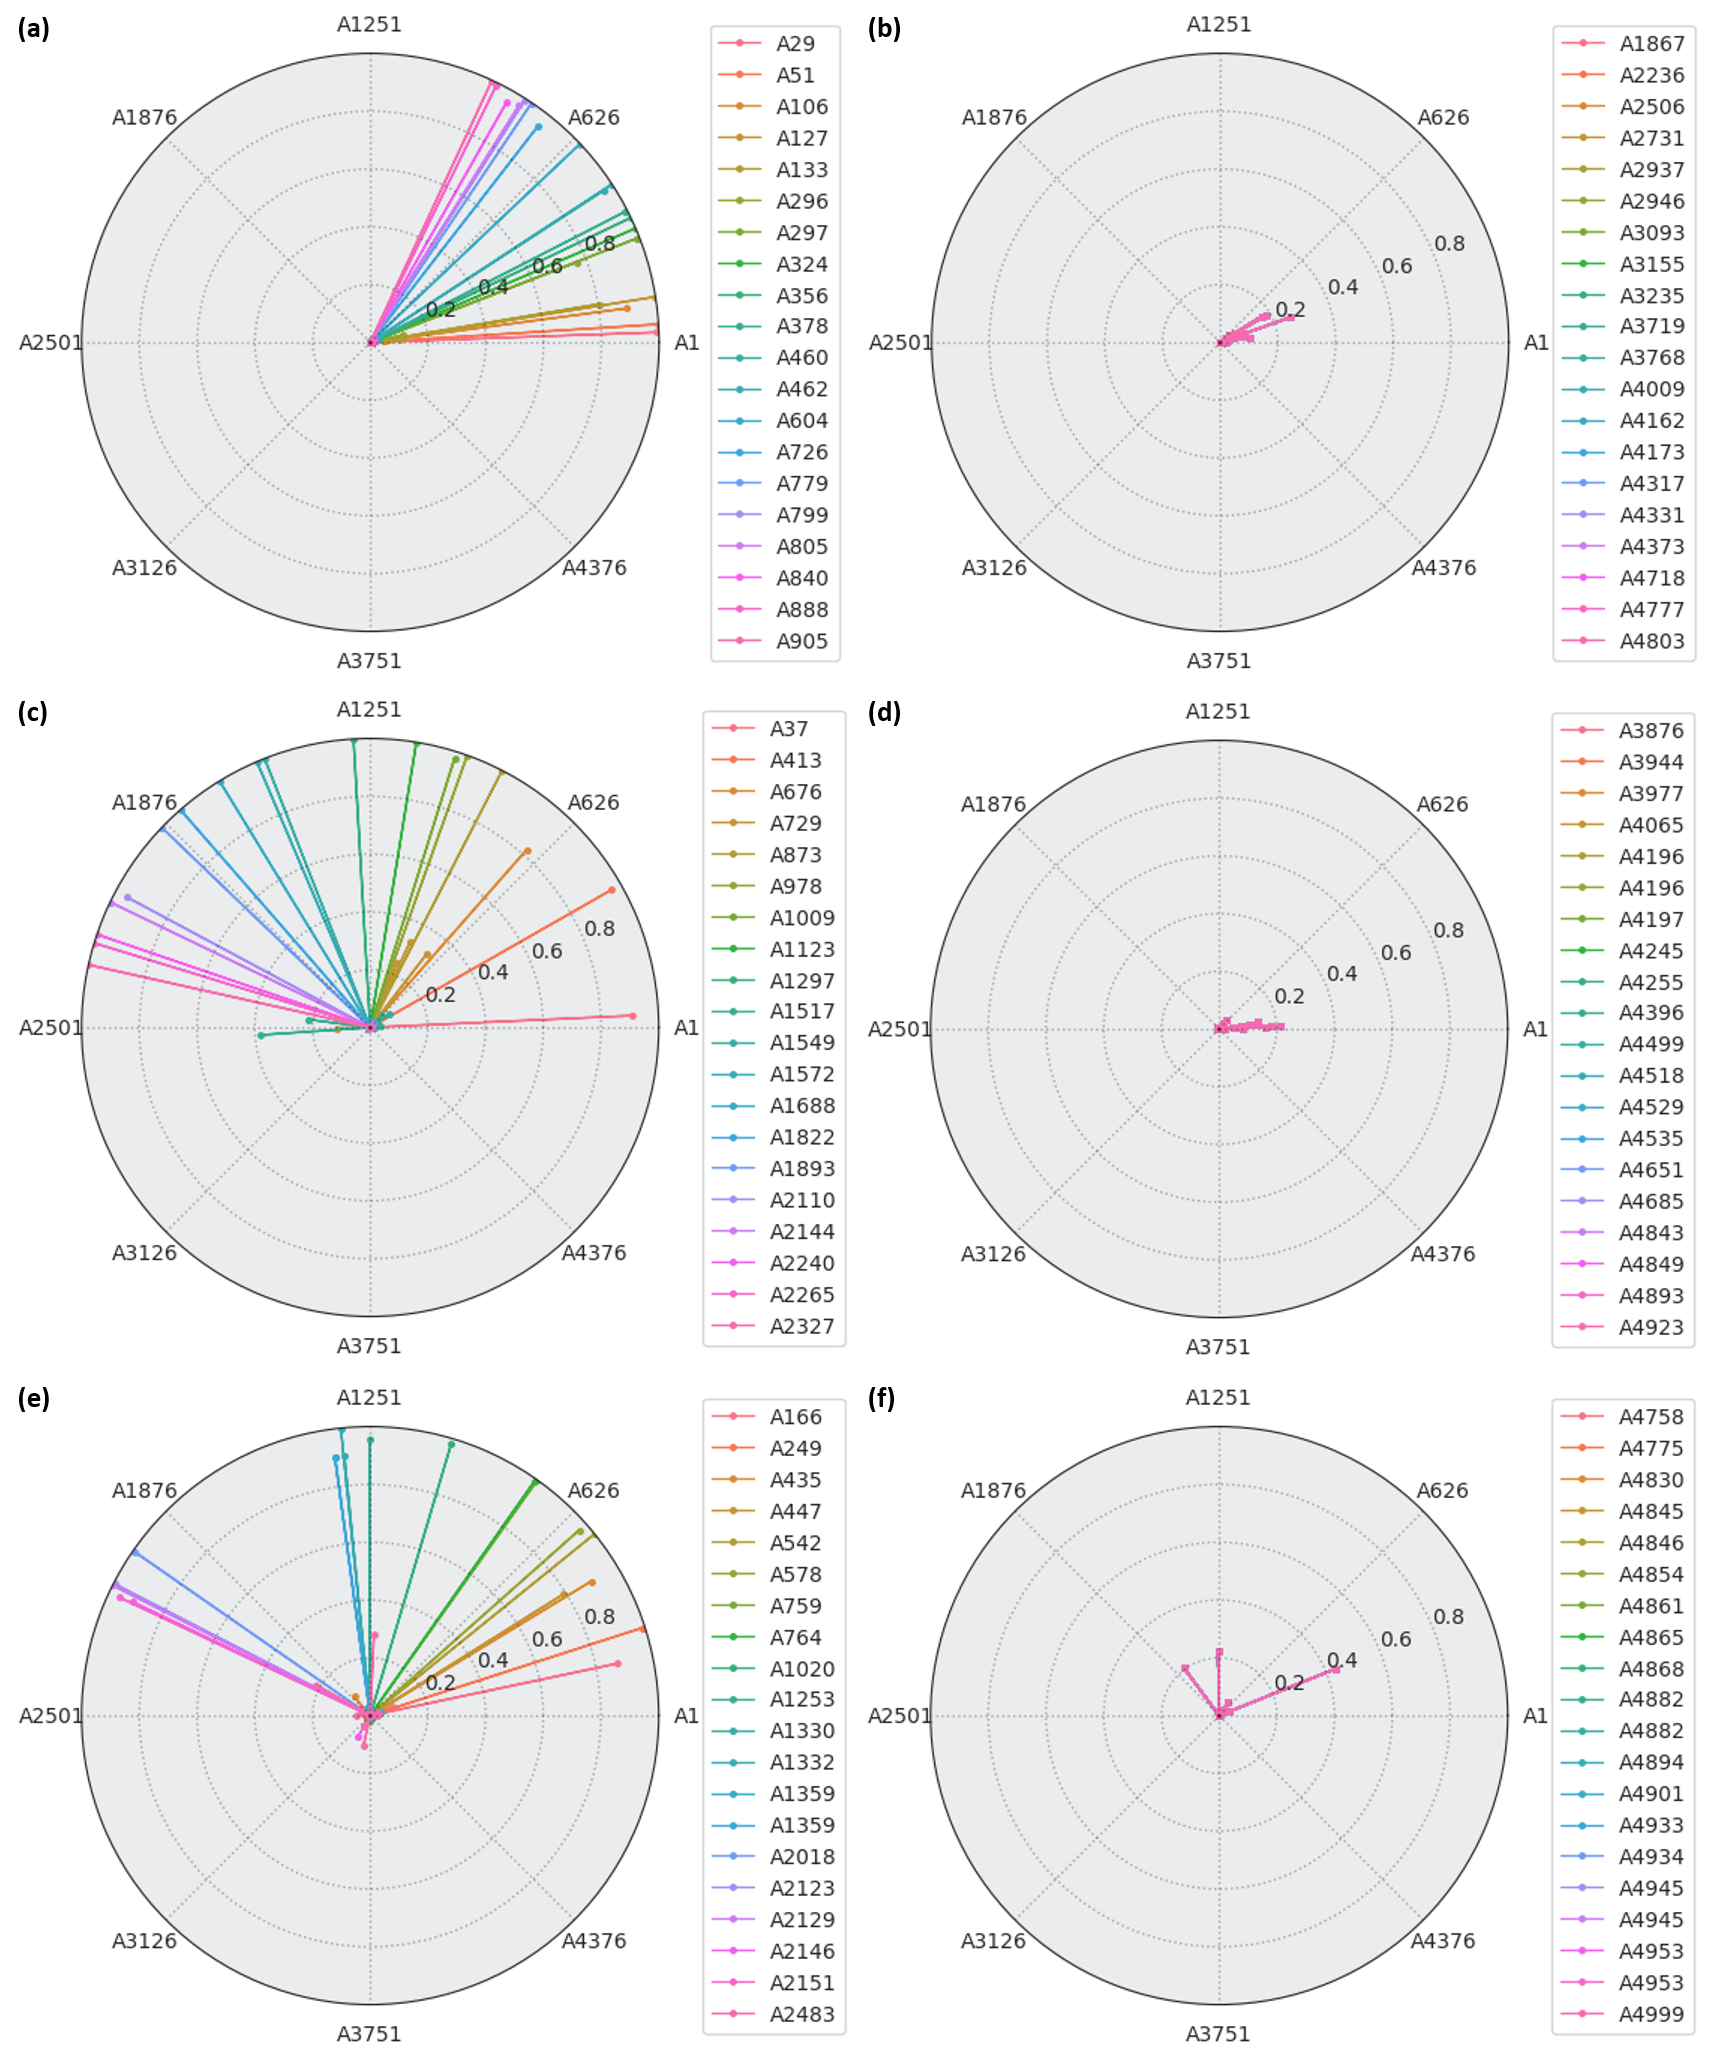
\includegraphics[width=0.8\textwidth]{allNPs_maxArchs_compareCloseMatch}
\caption{Radar plots indicating the contributions of all archetypes toward the samples that closely match the archetypes sampled from (a,c,e) those that lie outside the mainly empty sectors, and (b,d,f) those that lie within, for the (a-b) monometallic, (c-d) bimetallic, and (e-f) trimetallic nanoparticle datasets. ``A'' represents archetype.}
\label{fig:allNPs_maxArchs_compareCloseMatch}
\end{figure}
\begin{figure}[htbp!] \centering
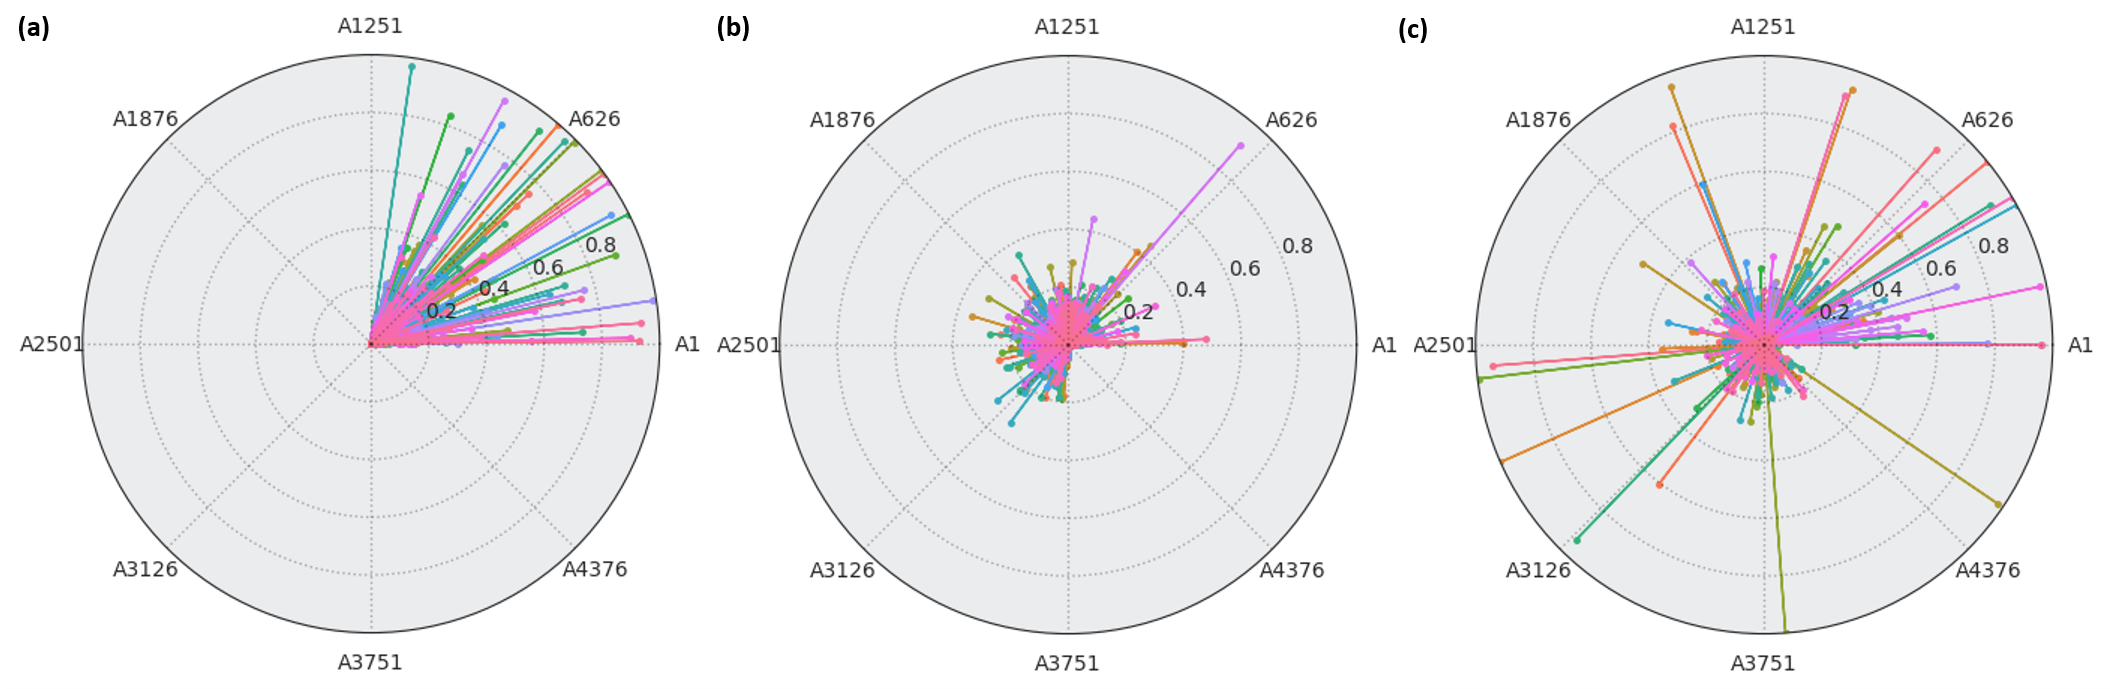
\includegraphics[width=\textwidth]{allNPs_maxArchs_compareArchContribRadarPlots}
\caption{Radar plots indicating the contributions of all archetypes toward 100 randomly sampled samples for the (a) monometallic, (b) bimetallic, and (c) trimetallic nanoparticle datasets. ``A'' represents archetype. The colours of lines indicate the order of the archetypes (the HSL colour palette of \texttt{seaborn} Python package is used, refer to Fig.~\ref{fig:allNPs_maxArchs_compareCloseMatch} for colour sequence).}
\label{fig:allNPs_maxArchs_compareArchContribRadarPlots}
\end{figure}

One likely explanation for the negligible contribution of the later archetypes is that they are near-duplicates of archetypes already returned earlier. The widely used \texttt{FurthestSum} initialisation~\cite{Morup2010furthestFirstAA} is known to have a tendency to include redundant archetypes when a large number of them is requested, because its early focus on suboptimal boundary points can trap the optimisation in poor local minima~\cite{Mair2023AA++}. Although the three-dimensional structures of the hypothetical archetypes cannot be directly visualised, their feature profiles can be examined as a proxy. As shown in Fig.~\ref{fig:allNPs_maxArchs_compareFeatProfRadarPlots_absent}, the feature profiles of later archetypes occupying the empty simplex regions are visually indistinguishable from one another across all features, providing clear confirmation of their redundancy.

\begin{figure}[htbp!] \centering
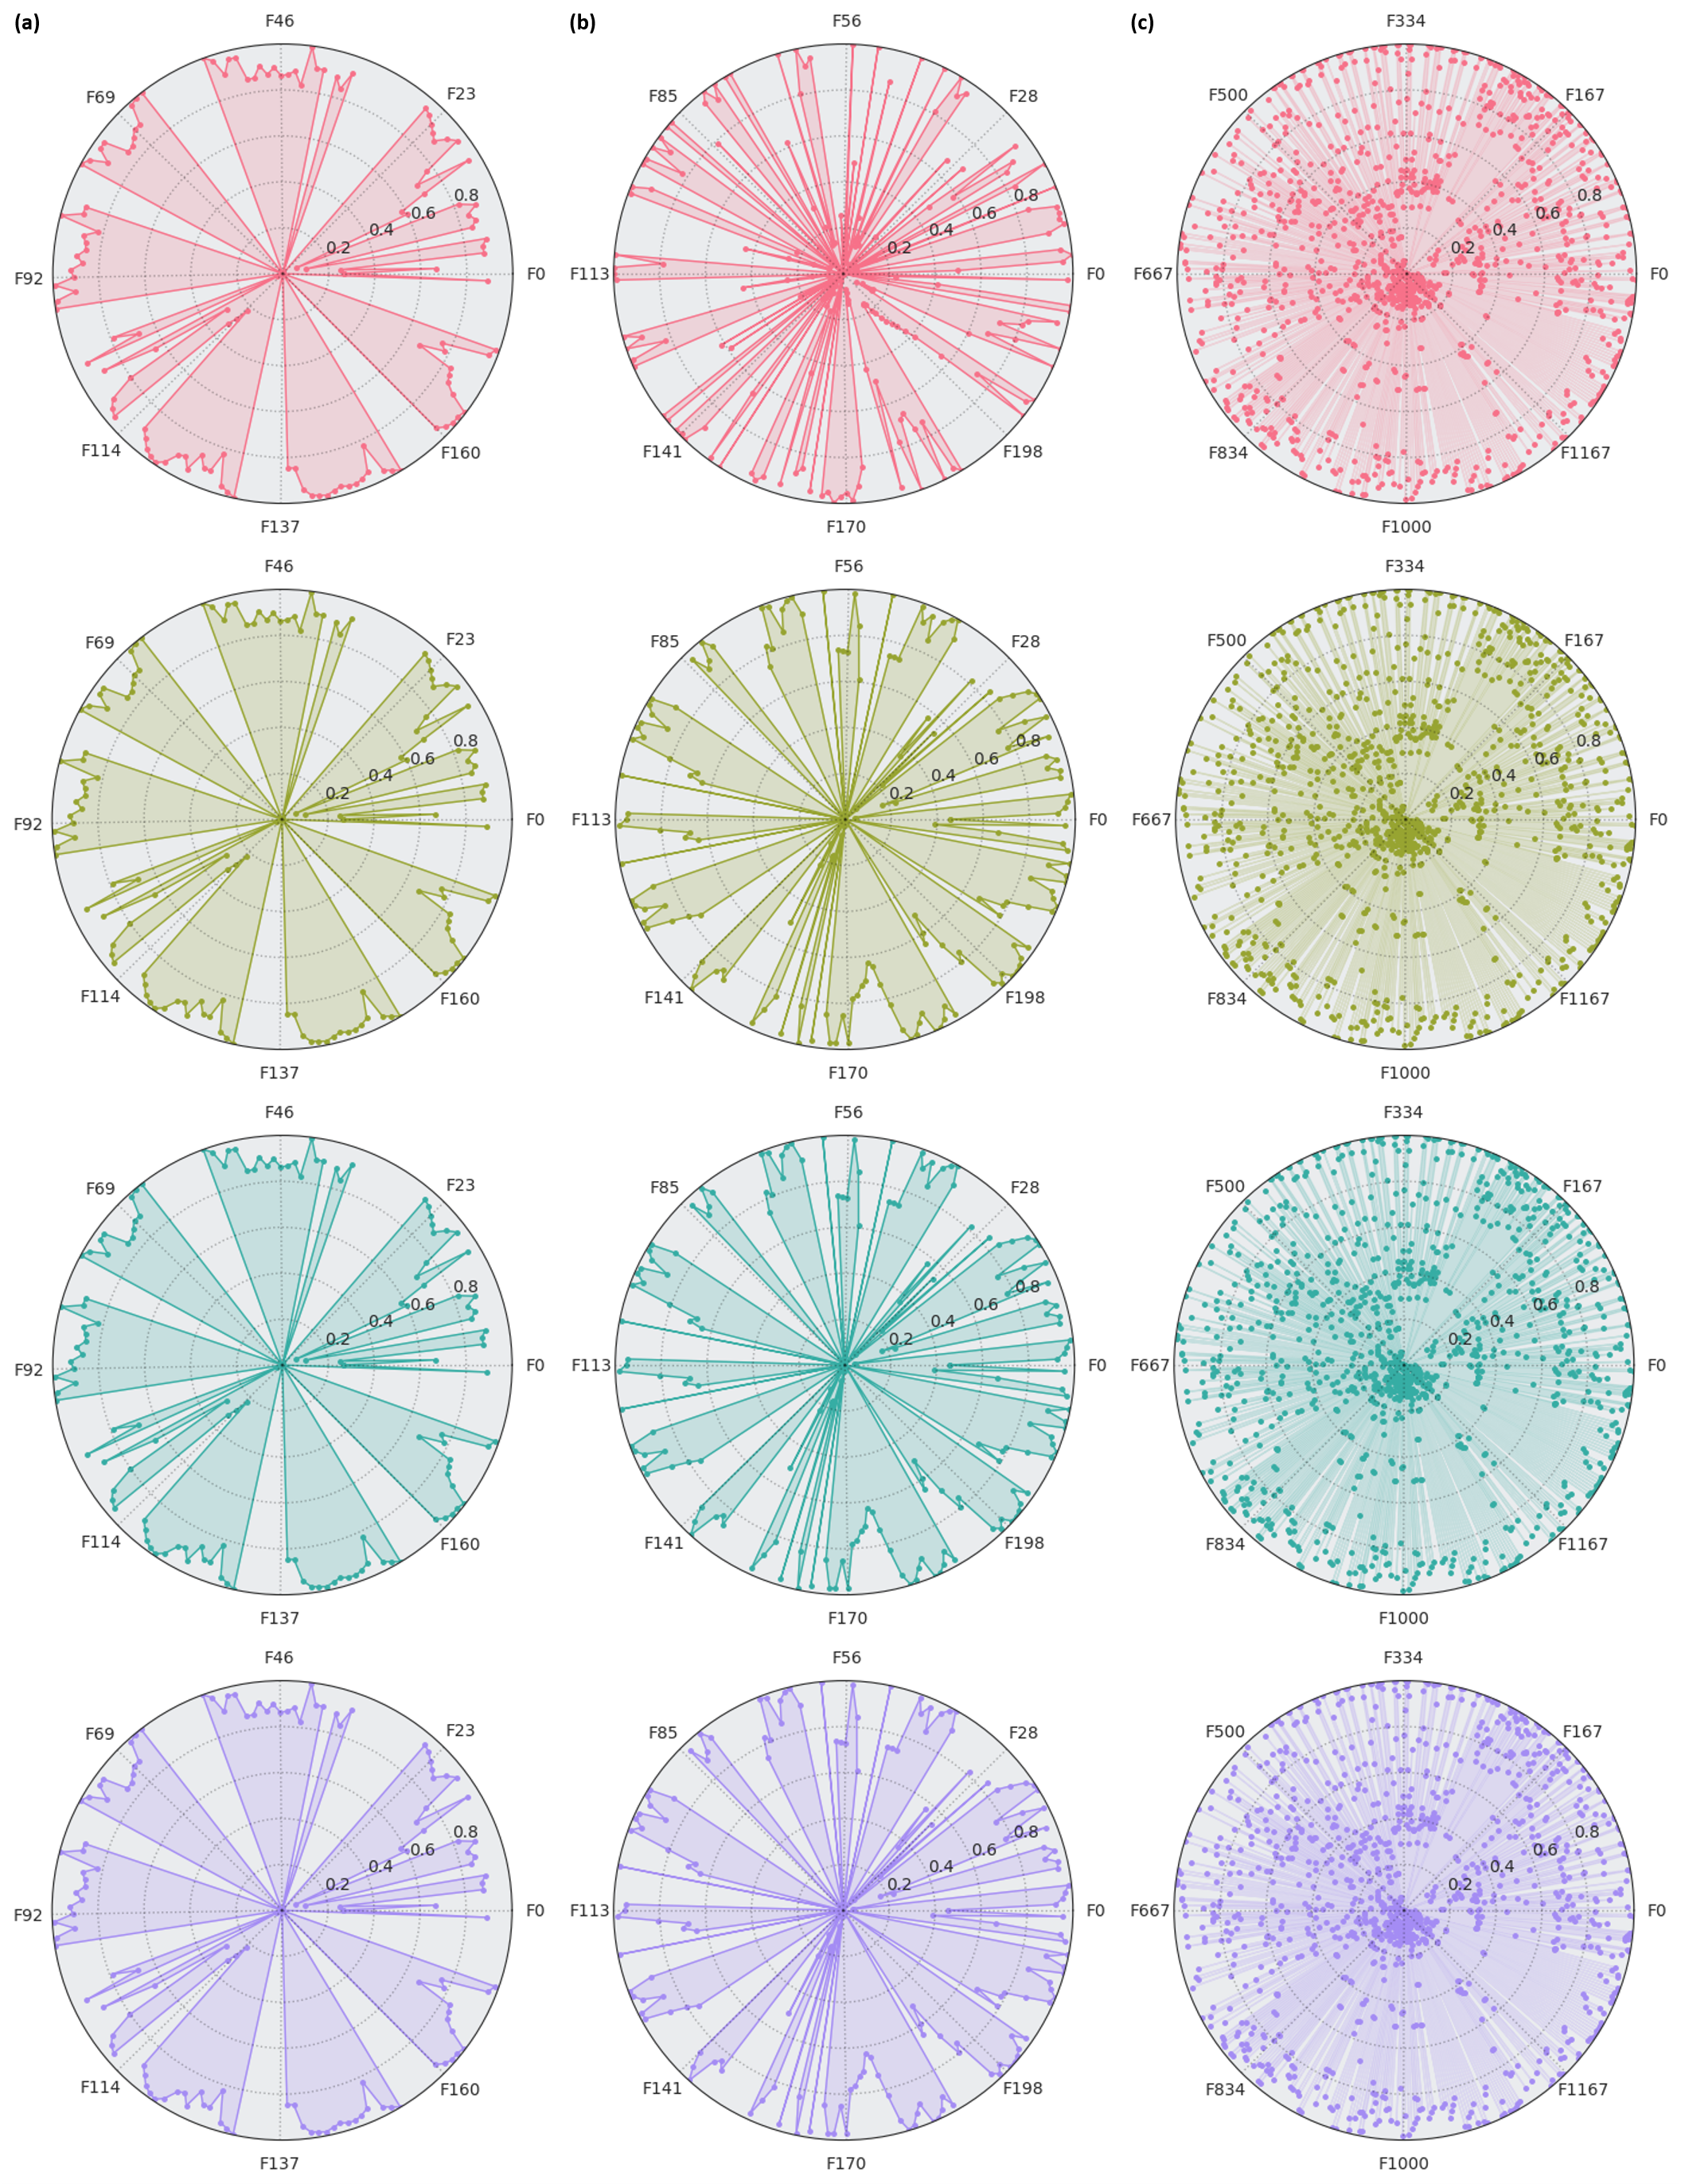
\includegraphics[width=0.95\textwidth]{allNPs_maxArchs_compareFeatProfRadarPlots_absent}
\caption{Radar plots displaying the feature profiles of archetypes from the mainly empty sectors of the simplex plots of the (a) monometallic, (b) bimetallic, and (c) trimetallic nanoparticle datasets.}
\label{fig:allNPs_maxArchs_compareFeatProfRadarPlots_absent}
\end{figure}



\clearpage
\section{Archetype Characterisation}
\label{sec:SIArchChar}

The feature profiles of the metallic nanoparticle archetypes can be examined through both radar and bar plot representations, as shown in Figs.~\ref{fig:allNPs_featProf} and~\ref{fig:allNPs_maxArchs_compareFeatProfRadarPlots_actual}. Radar plots are well suited for simultaneously comparing the full feature set across several archetypes, while bar plots are more practical for detailed inspection of a selected subset of features.

\begin{figure}[h] \centering
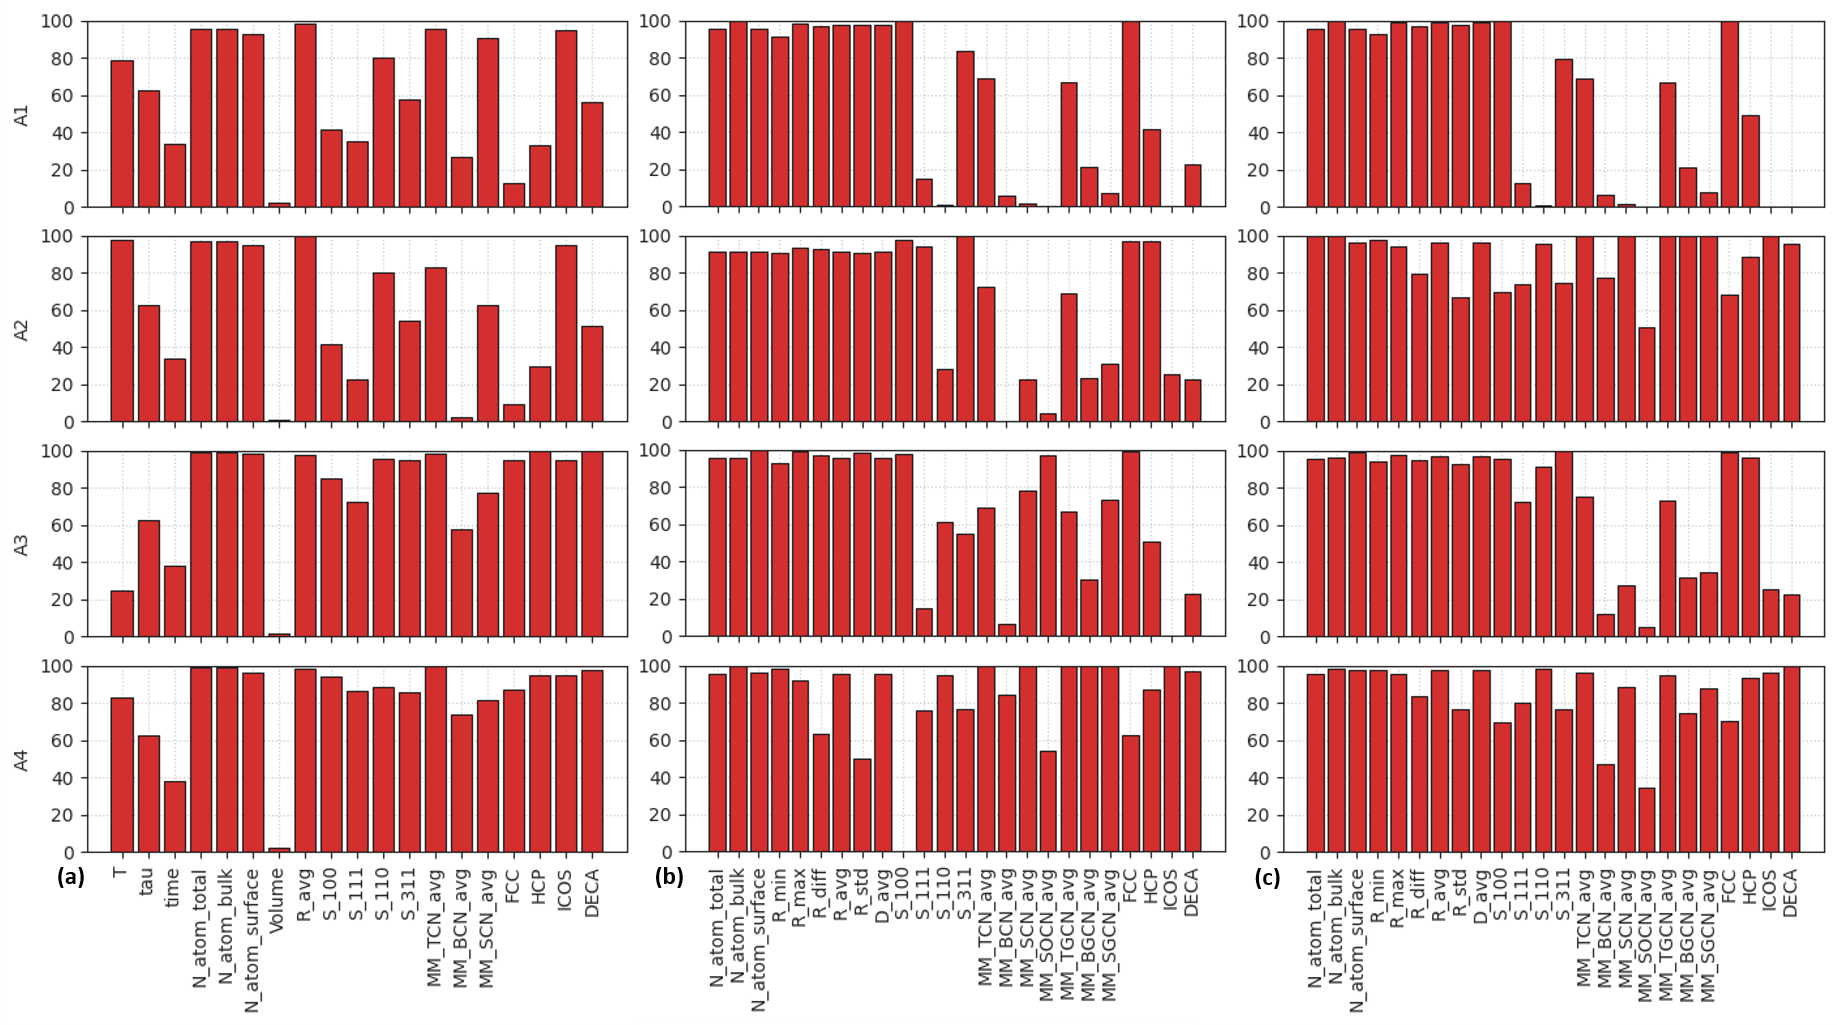
\includegraphics[width=\textwidth]{allNPs_featProf}
\caption{Bar plots of feature profiles for archetypes 1-4 from archetypal analysis of (a) monometallic, (b) bimetallic, and (c) trimetallic nanoparticle datasets. ``A" represents archetype.}
\label{fig:allNPs_featProf}
\end{figure}

\begin{figure} \centering
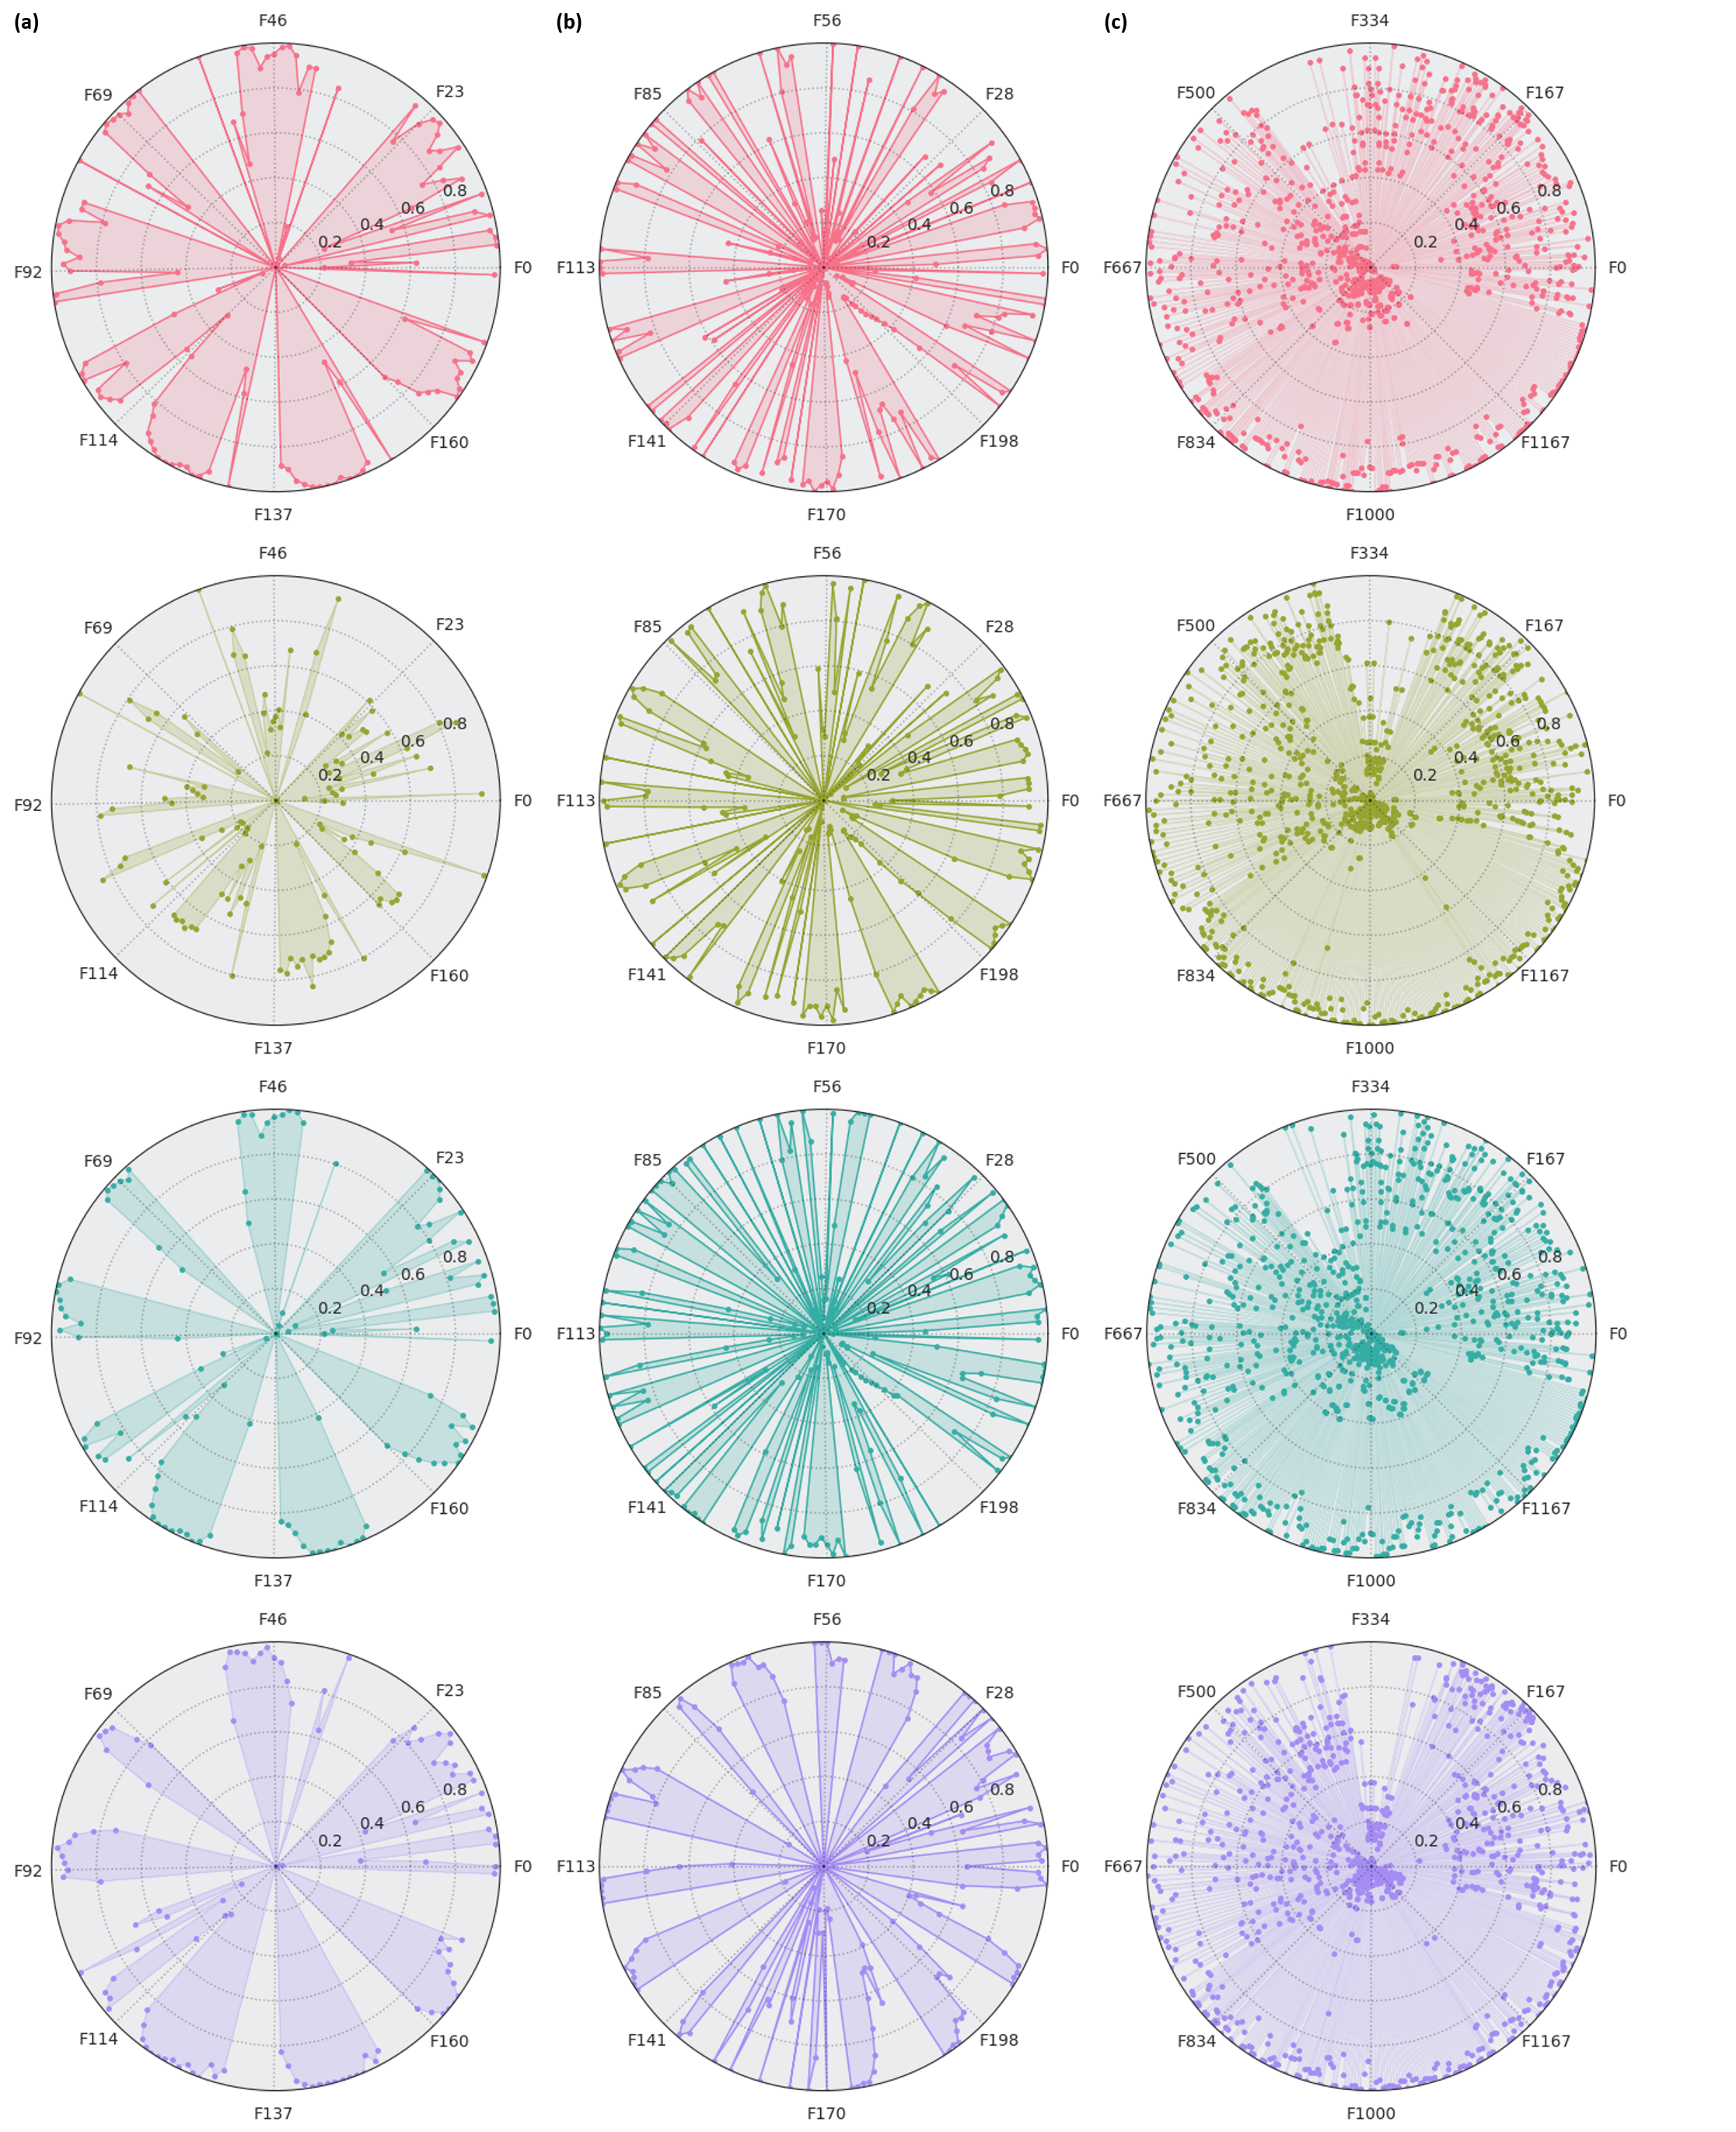
\includegraphics[width=\textwidth]{allNPs_maxArchs_compareFeatProfRadarPlots_actual}
\caption{Radar plots of feature profiles for archetypes 1 (red), 2 (yellow), 3 (turquoise), and 4 (purple) from archetypal analysis of (a) monometallic, (b) bimetallic, and (c) trimetallic nanoparticle datasets. ``F" represents feature.}
\label{fig:allNPs_maxArchs_compareFeatProfRadarPlots_actual}
\end{figure}



\clearpage
\section{Linear Regression Results on Energy Prediction}
\label{sec:SILRRRes}

The learning curves and evaluation results for the fitted linear regressors are shown in Figure~\ref{fig:LRRresultsEtotform}. For total energy prediction, the model trained on the most archetypal samples achieved $R^2$ scores of 0.995 (training), $0.981 \pm 0.004$ (cross-validation), and 0.972 (testing). These are comparable to the scores obtained using all training samples: 0.981 (training), $0.981 \pm 0.002$ (cross-validation), and 0.979 (testing). For formation energy prediction, the archetypal-sample model achieved $R^2$ scores of 0.977 (training), $0.927 \pm 0.023$ (cross-validation), and 0.928 (testing), compared with 0.957 (training), $0.956 \pm 0.003$ (cross-validation), and 0.959 (testing) when all training samples are used.

\begin{figure}[htbp]
    \centering
    \footnotesize
    \begin{subfigure}{0.4\textwidth}
        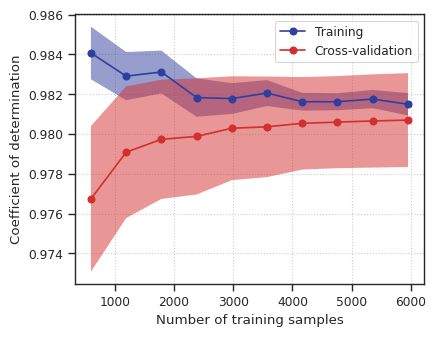
\includegraphics[width=\textwidth]{MNPELearnCurveLRR_Etot_minmax}
        \caption{} \label{fig:MNPELearnCurveLRR_Etot_minmax}
    \end{subfigure}
    \begin{subfigure}{0.41\textwidth}
        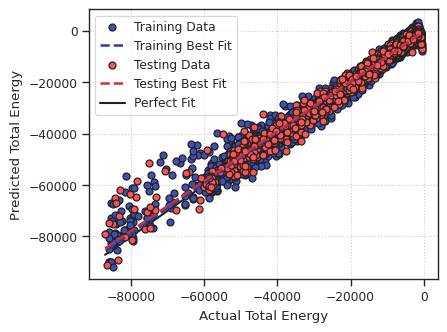
\includegraphics[width=\textwidth]{MNPR2AllLRR_Etot_minmax}
        \caption{} \label{fig:MNPER2AllLRR_Etot_minmax}
    \end{subfigure}
    \begin{subfigure}{0.41\textwidth}
        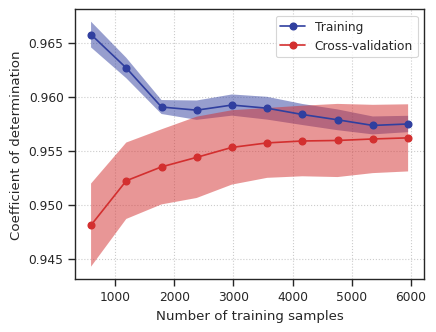
\includegraphics[width=\textwidth]{MNPELearnCurveLRR_Eform_minmax}
        \caption{} \label{fig:MNPELearnCurveLRR_Eform_minmax}
    \end{subfigure}
    \begin{subfigure}{0.41\textwidth}
        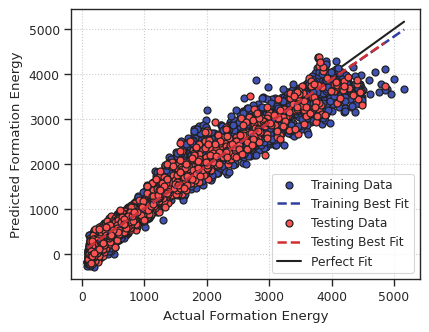
\includegraphics[width=\textwidth]{MNPR2AllLRR_Eform_minmax}
        \caption{} \label{fig:MNPER2AllLRR_Eform_minmax}
    \end{subfigure}
    \begin{subfigure}{0.39\textwidth}
        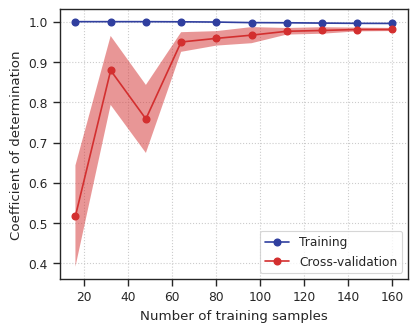
\includegraphics[width=\textwidth]{MNPELearnCurveLRR_red_Etot_minmax}
        \caption{} \label{fig:MNPELearnCurveLRR_red_Etot_minmax}
    \end{subfigure}
    \begin{subfigure}{0.41\textwidth}
        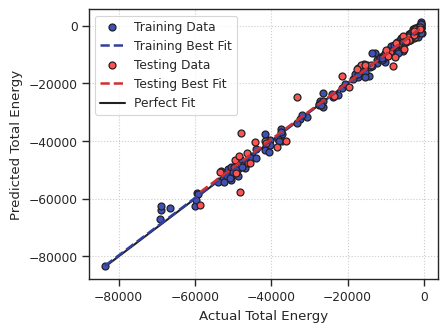
\includegraphics[width=\textwidth]{MNPR2AllLRR_red_Etot_minmax}
        \caption{} \label{fig:MNPR2AllLRR_red_Etot_minmax}
    \end{subfigure}
    \begin{subfigure}{0.41\textwidth}
        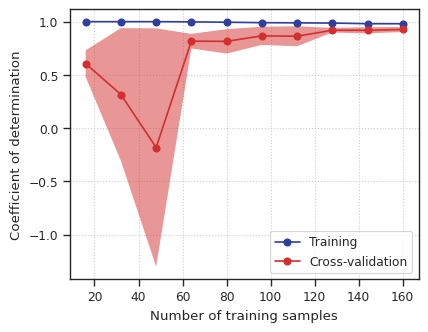
\includegraphics[width=\textwidth]{MNPELearnCurveLRR_red_Eform_minmax}
        \caption{} \label{fig:MNPELearnCurveLRR_red_Eform_minmax}
    \end{subfigure}
    \begin{subfigure}{0.41\textwidth}
        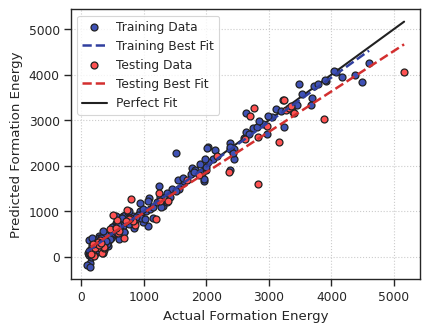
\includegraphics[width=\textwidth]{MNPR2AllLRR_red_Eform_minmax}
        \caption{} \label{fig:MNPR2AllLRR_red_Eform_minmax}
    \end{subfigure}
    \caption{Results of the optimised linear regressors fitted to (a-d) all training samples and (e-h) most archetypal samples, predicting the (a-b, e-f) total energy and (c-d, g-h) formation energy of monometallic nanoparticles: (a, c, e, g) learning curves and (b, d, f, h) scatter plots of predictions on training and testing sets.}
    \label{fig:LRRresultsEtotform}
\end{figure}

For linear regressors trained on randomly selected samples of equal size, the average $R^2$ scores for total energy prediction were 0.989 (training), $0.949 \pm 0.027$ (validation), and 0.969 (testing). For formation energy, the corresponding averages were 0.975 (training), $0.898 \pm 0.037$ (validation), and 0.911 (testing). Consistent with the random forest results reported in the main text, models trained on randomly selected samples of equivalent size were uniformly outperformed by those trained on IAA-selected archetypal samples.



% ---- Bibliography ----
\clearpage
\bibliographystyle{unsrt}
\bibliography{ref.bib}


\end{document}
